% Source: graduate-coursework/Research/Intro_to_Agents/handouts/Part8_Advanced_Topics.tex

\documentclass[border=4pt]{standalone}
\usepackage[T1]{fontenc}
\usepackage{graphicx}
\usepackage{lmodern}
\usepackage{tikz}
\usepackage{xcolor}
\usetikzlibrary{shapes.geometric, arrows.meta, positioning, calc, fit, backgrounds, matrix, decorations.pathreplacing}

\definecolor{UofSCGarnet}{HTML}{73000a}
\definecolor{UofSCBlack}{HTML}{000000}
\definecolor{UofSCWhite}{HTML}{ffffff}
\definecolor{UofSCRose}{HTML}{CC2E40}
\definecolor{UofSCAtlantic}{HTML}{466A9F}
\definecolor{UofSCCongaree}{HTML}{1F414D}
\definecolor{UofSCHorseshoe}{HTML}{65780B}
\definecolor{UofSCGrass}{HTML}{CED318}
\definecolor{UofSCHoneycomb}{HTML}{A49137}
\definecolor{UofSC90Black}{HTML}{363636}
\definecolor{UofSC70Black}{HTML}{5C5C5C}
\definecolor{UofSC50Black}{HTML}{A2A2A2}
\definecolor{UofSCWarmGrey}{HTML}{676156}
\definecolor{UofSCSandstorm}{HTML}{FFF2E3}
\definecolor{UofSCDarkGarnet}{HTML}{570008}
\definecolor{UofSCAzalea}{HTML}{844247}

\tikzset{
    % Sharp corners for all nodes
    every node/.style={font=\small},
    % Process box style
    process/.style={
        rectangle,
        draw=UofSCBlack,
        fill=UofSCWhite,
        minimum width=2.5cm,
        minimum height=0.8cm,
        align=center,
        font=\footnotesize
    },
    % Decision box style
    decision/.style={
        diamond,
        draw=UofSCBlack,
        fill=UofSCSandstorm,
        minimum width=2cm,
        minimum height=1cm,
        align=center,
        font=\footnotesize,
        aspect=2
    },
    % Start/End style
    startstop/.style={
        rectangle,
        draw=UofSCGarnet,
        fill=UofSCGarnet,
        text=UofSCWhite,
        minimum width=2cm,
        minimum height=0.7cm,
        align=center,
        font=\footnotesize\bfseries
    },
    % Arrow style
    arrow/.style={
        ->,
        >=Stealth,
        thick,
        color=UofSCBlack
    },
    % Failure node
    failure/.style={
        rectangle,
        draw=UofSCRose,
        fill=UofSCRose!20,
        minimum width=2cm,
        minimum height=0.7cm,
        align=center,
        font=\footnotesize
    },
    % Success node
    success/.style={
        rectangle,
        draw=UofSCHorseshoe,
        fill=UofSCHorseshoe!20,
        minimum width=2cm,
        minimum height=0.7cm,
        align=center,
        font=\footnotesize
    },
    % Highlight box
    highlight/.style={
        rectangle,
        draw=UofSCGarnet,
        fill=UofSCGarnet!10,
        line width=1.5pt,
        minimum width=2.5cm,
        minimum height=0.8cm,
        align=center,
        font=\footnotesize
    },
    % Security threat style
    threat/.style={
        rectangle,
        draw=UofSCRose,
        fill=UofSCRose!15,
        minimum width=2.2cm,
        minimum height=0.7cm,
        align=center,
        font=\footnotesize
    },
    % Agent node
    agent/.style={
        rectangle,
        draw=UofSCAtlantic,
        fill=UofSCAtlantic!15,
        minimum width=2.2cm,
        minimum height=0.8cm,
        align=center,
        font=\footnotesize
    },
    % Human node
    human/.style={
        rectangle,
        draw=UofSCCongaree,
        fill=UofSCCongaree!15,
        minimum width=2.2cm,
        minimum height=0.8cm,
        align=center,
        font=\footnotesize
    },
    % Cost node
    cost/.style={
        rectangle,
        draw=UofSCHoneycomb,
        fill=UofSCHoneycomb!20,
        minimum width=2cm,
        minimum height=0.7cm,
        align=center,
        font=\footnotesize
    },
    % Test node
    test/.style={
        rectangle,
        draw=UofSCAtlantic,
        fill=UofSCAtlantic!10,
        minimum width=2cm,
        minimum height=0.7cm,
        align=center,
        font=\footnotesize
    },
    % Pipeline stage
    pipeline/.style={
        rectangle,
        draw=UofSCCongaree,
        fill=UofSCCongaree!10,
        minimum width=2.5cm,
        minimum height=0.8cm,
        align=center,
        font=\footnotesize
    },
    % Timeline event
    timeline/.style={
        rectangle,
        draw=UofSCGarnet,
        fill=UofSCWhite,
        minimum width=1.8cm,
        minimum height=0.6cm,
        align=center,
        font=\tiny
    }
}

\begin{document}
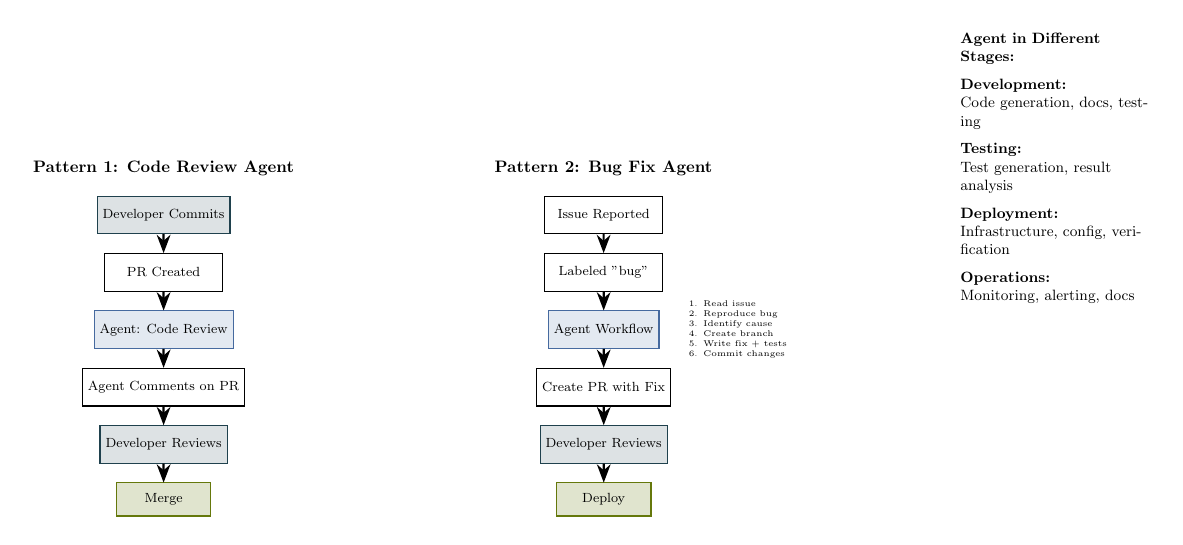
\begin{tikzpicture}[node distance=0.4cm and 1cm, scale=0.6, transform shape]
        % Code Review Agent Pattern
        \node (title1) [font=\bfseries] {Pattern 1: Code Review Agent};
        \node (dev) [human, below=0.3cm of title1] {Developer Commits};
        \node (pr) [process, below=of dev] {PR Created};
        \node (agent1) [agent, below=of pr] {Agent: Code Review};
        \node (comment) [process, below=of agent1] {Agent Comments on PR};
        \node (review) [human, below=of comment] {Developer Reviews};
        \node (merge) [success, below=of review] {Merge};

        \draw [arrow] (dev) -- (pr);
        \draw [arrow] (pr) -- (agent1);
        \draw [arrow] (agent1) -- (comment);
        \draw [arrow] (comment) -- (review);
        \draw [arrow] (review) -- (merge);

        % Bug Fix Agent Pattern
        \node (title2) [font=\bfseries, right=4cm of title1] {Pattern 2: Bug Fix Agent};
        \node (issue) [process, below=0.3cm of title2] {Issue Reported};
        \node (label) [process, below=of issue] {Labeled "bug"};
        \node (agent2) [agent, below=of label] {Agent Workflow};
        \node (fix) [process, below=of agent2] {Create PR with Fix};
        \node (dev2) [human, below=of fix] {Developer Reviews};
        \node (deploy) [success, below=of dev2] {Deploy};

        \draw [arrow] (issue) -- (label);
        \draw [arrow] (label) -- (agent2);
        \draw [arrow] (agent2) -- (fix);
        \draw [arrow] (fix) -- (dev2);
        \draw [arrow] (dev2) -- (deploy);

        % Agent workflow details
        \node [right=0.5cm of agent2, font=\tiny, text width=2.5cm] {
            1. Read issue\\
            2. Reproduce bug\\
            3. Identify cause\\
            4. Create branch\\
            5. Write fix + tests\\
            6. Commit changes
        };

        % Agent stages
        \node [right=5cm of title2, text width=4cm, font=\small] {
            \textbf{Agent in Different Stages:}\\[0.2cm]
            \textbf{Development:}\\
            Code generation, docs, testing\\[0.2cm]
            \textbf{Testing:}\\
            Test generation, result analysis\\[0.2cm]
            \textbf{Deployment:}\\
            Infrastructure, config, verification\\[0.2cm]
            \textbf{Operations:}\\
            Monitoring, alerting, docs
        };
    \end{tikzpicture}
\end{document}
